\subsubsection{Communication Port}

The communication port is the only component needed to defined a communication layer of the service.
It encapsulates detail needed to express a service, which are the listening protocol, location, and the interfaces. The location of port defines the communication channel for the port. For protocol part, Jolie supports variety of communication protocol, not only limited to the web protocol like SOAP, HTTP and, SODEP (a Jolie specific binary protocol), it is also supports bluetooth protocol and the in-memory protocol. Lastly, the interfaces defines a list of operations related to the port depending on type of the port.

Communication port in Jolie can be classified into two types, whether it is exposing a communication channel to the external service so called an \textit{inputPort}, or it is expressing the communication channel to other service, or the \textit{outputPort}.

Jolie also equipped with the primitives to define the advance composition of the input port. One of the primitive that is offered by Jolie is \textit{aggregation}, Aggregation composes operations from a output port to defining input port, allows a the input port accepts operations express in output port and developer is able to intercept a message.

\begin{figure}[ht]
    \begin{framed}
        \begin{grammar}

            <outputPort> ::= `outputPort' \\ <portName> `{' <portConfigurationPair>+ `}'

            <inputPort>
            ::= `inputPort' <portName> `{' ( <portConfigurationPair> | <inputPortConfigurationPair> )+ `}'

            <portConfigurationPair>
            ::= `location' `:' \textit{StringLiteral}
            \alt `protocol' `:' <ID>
            \alt `interfaces' `:' <interfaceName>

            <inputPortConfigurationPair>
            ::=  `aggregates' `:' <portName> ( `,' <portName> )* \alt \dots

            <portName> ::= <ID>
            <interfaceName> ::= <ID>

        \end{grammar}
    \end{framed}
    \caption{Jolie Port Definition Syntax}
\end{figure}

\FloatBarrier

For an example of this section, we create a service as depicted at ~\ref{list:example-port-graphic}.
The service \texttt{program} acts as a producer of the operations in \texttt{personInterface}, where the communication channel is defined in \texttt{personInputPort}.
This service is also acted as a consumer of \texttt{loggerInterface} defined by an output port \texttt{LoggerOutputPort}.
One key takeaway from this example is aggregation at line 11 makes \texttt{personInputPort} accepts additional operation defined in the \texttt{personInterface}. There are different scenarios which altered the behavior when the client invoke an aggregated operation. For this specific example, since the operations in \texttt{loggerInterface} are distinct to interface defined in the input port, Jolie will automatically forward the message to the origin aggregation output port.

For the interaction between ports through input/output operations which we will look at it again in ~\ref{sec:jolie-behavior}.

\begin{figure}[ht]
    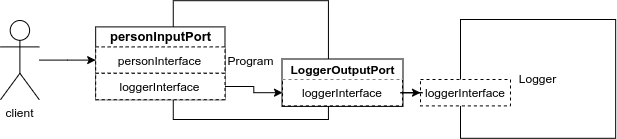
\includegraphics[width=10cm]{ExamplePort}
    \centering
    \caption{A service for port example}
    \label{list:example-port-graphic}
\end{figure}

\begin{listing}[ht]

    \lstset{language=Jolie,
        style=codeStyle,
        numbers=left,
        firstnumber=1
    }
    \begin{lstlisting}[frame=tlrb, caption= {Jolie Port declaration example}, label={list:example-port} ]{port-Jolie}
outputPort LoggerOutputPort {
    location: "socket://logger-service-location:3000"
    protocol: sodep
    interfaces: loggerInterface
}

inputPort personInputPort {
    location: "socket://localhost:3000"
    protocol: http
    interfaces: personInterface
    aggregates: Logger
}

main {
    createPerson(person)(result){
        log@LoggerOutputPort(person)
        result = true
    }
}
\end{lstlisting}
\end{listing}

\FloatBarrier
